\section{Incident Source Conditions}
Primarily there are two kinds of sources in FDTD: point sources and plane wave sources.

Point source can be classified as hard source or soft source. If the source value is directly assigned to the certain
point, this is referred to as a hard source. Oppositely, it can be called a soft source if the source value is added to
the field at that point. A hard source would lead to some reflection between certain points and adjacent points and a
soft source allows wave just pass through. Point source is not common used in 2D and 3D simulation but play a important
role on constructing plane wave source conditions.

For investigating nano structures, it's often of interest to impinge plane wave source upon structures and measure
transmission and reflection. The calculation of radar cross section also deals with plane wave. Total Field / Scatter
Field (TFSF) is a technique to to simulate a plane wave by dividing problem space into Totol Field region and Scatter
Field region(Fig.\ref{fig:tfsf}).
\begin{center}\label{fig:tfsf}
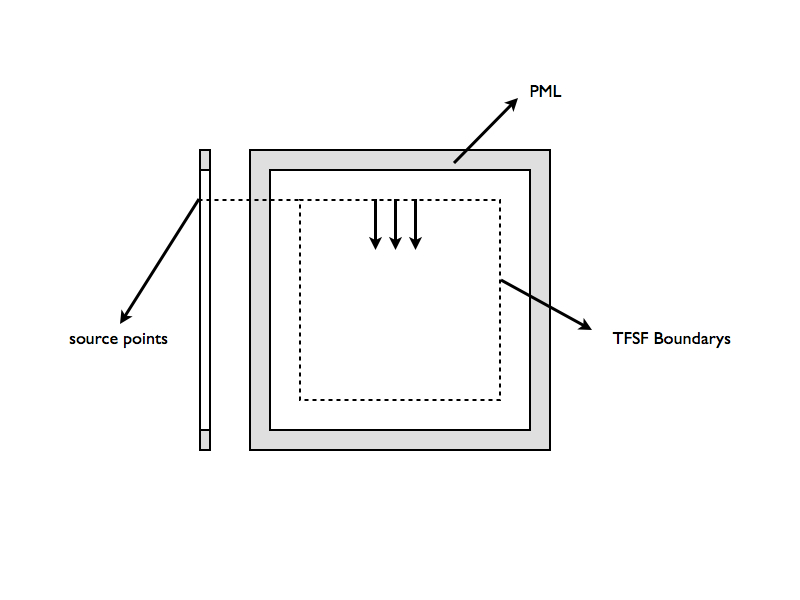
\includegraphics[scale=0.5]{images/tfsf.jpg}
\end{center}
The TFSF formulas can be observed through complete update equation and totol/scatter field theory as
\begin{displaymath}\label{eq:e_ts}
  E_{total}=E_{scatter}+E_{incident}
\end{displaymath}
\begin{displaymath}\label{eq:h_ts}
  H_{total}=H_{scatter}+H_{incident}  
\end{displaymath}
By example of the Y incident plane wave of TM polarization in TFSF region $x=ia:ib, y=ja:jb, z=ka:kb$, Eq.\ref{eq:dz3d}
performed on edage $y=ja$ of main computation domain is actually 
\begin{equation}
  \begin{split}
    \widetilde{D}_{z,total}|_{i,ja,k} = \widetilde{D}_{z,total}|_{i,ja,k} &+ 0.5 \cdot \left( H_{y,total}|_{i+\frac{1}{2},ja,k+\frac{1}{2}} - H_{y,total}|_{i-\frac{1}{2},ja,k+\frac{1}{2}} \right) \\
    &- 0.5 \cdot \left( H_{x,total}|_{i,ja+\frac{1}{2},k+\frac{1}{2}} - H_{x,scatter}|_{i,ja-\frac{1}{2},k+\frac{1}{2}} \right)    
  \end{split}
\end{equation}
Remark the last $H_x$ belongs to scatter field outside the TFSF boundary. By applying Eq.\ref{eq:h_ts} to complete the
curl operation, the insertion of TFSF source of $\widetilde{D}_z$ is described as following.
\begin{displaymath}
  \widetilde{D}_z|_{i,ja,k} = \widetilde{D}_z|_{i,ja,k} + 0.5 \cdot H_{inc}|_{ja-\frac{1}{2}}
\end{displaymath}
The rest insertion of TFSF can also be dervied.
\begin{displaymath}
  \widetilde{D}_z|_{i,jb,k} = \widetilde{D}_z|_{i,jb,k} - 0.5 \cdot H_{inc}|_{jb+\frac{1}{2}}  
\end{displaymath}
\begin{displaymath}
  \widetilde{B}_x|_{i,ja-\frac{1}{2},k+\frac{1}{2}}=\widetilde{B}_x|_{i,ja-\frac{1}{2},k+\frac{1}{2}}+0.5 \cdot E_{inc}|_{ja}
\end{displaymath}
\begin{displaymath}
  \widetilde{B}_x|_{i,jb+\frac{1}{2},k+\frac{1}{2}}=\widetilde{B}_x|_{i,jb+\frac{1}{2},k+\frac{1}{2}}-0.5 \cdot E_{inc}|_{jb}
\end{displaymath}
\begin{displaymath}
  \widetilde{B}_y|_{ia-\frac{1}{2},ja:jb,k+\frac{1}{2}}=\widetilde{B}_y|_{ia-\frac{1}{2},ja:jb,k+\frac{1}{2}}-0.5 \cdot E_{inc}|_{ja:jb}
\end{displaymath}
\begin{displaymath}
  \widetilde{B}_y|_{ib+\frac{1}{2},ja:jb,k+\frac{1}{2}}=\widetilde{B}_y|_{ib+\frac{1}{2},ja:jb,k+\frac{1}{2}}+0.5 \cdot E_{inc}|_{ja:jb}
\end{displaymath}






